\documentclass{article}
\usepackage{epsfig}
\usepackage{amsmath}
\usepackage{amsfonts}
\usepackage{amssymb}

%\def\labexe{Expt361}

%\def\expttitle{RC and LC filters}
%\def\exptnumber{361}

%\newcommand{\IsDocumentReady}{True}
%\newcommand{\IsExperiment}{True}

%\newcommand{\expcolor}{B} % R,G,B.
%\newcommand{\ELF}{4}

%\usepackage{minted}
%\usepackage{399}
\usepackage[a4paper, total={6.5in, 9.5in}]{geometry}

\begin{document}

\title{Experiment 361}
\author{ }
\maketitle

\section*{Aim}
The responses of resistors, capacitors and inductors to (varying)
input voltages/currents can filter or amplify these input
signals. Such circuits are commonly used in the electronics you use
every day. This lab lets you investigate the theoretical properties of
passive RC and LC filters, and to experimentally verify these
properties.

{\bf As in all advanced lab experiments, the questions posed in this
handout merely serve as a guidance to write your comprehensive lab
report.}

\section*{Reference}
The best reference book for this lab is the stage 2 Physics 240 text
(OR IS IT 340? 244?): "Linear steady state network theory" by
G.E.J. Bold and J. B. Earnshaw. {\bf should we make this available
  somewhere?}

For more a detailed analysis of the Bode and Nyquist plots of passive
circuits try "Network analysis and synthesis" by Franklin Kuo, or any
of the many other electronics texts available in the library. {\bf Do
  we have something less than 50 years old for these students?}
 
\section*{Introduction}
In electronics, filters are circuits which perform signal processing
functions to either remove or enhance certain frequency
components. Filters can be classified as either active or passive,
with active filters usually containing amplifying components in the
circuit and requiring an external power source. In this experiment we
shall study passive filters based on combinations of resistors,
inductors and capacitors. 

\section*{Theory}
One way to define a certain type of filter is to consider the ratio of
the output to the input voltage. This ratio is called the transfer
function
\begin{equation}
  \mathbf{T}(f)=\frac{\mathbf{V}_{out}(f)}{\mathbf{V}_{in}(f)}.
\end{equation}
% As we are dealing with AC signals in circuits containing inductors
% and resistors, the voltage transfer function will be a complex
% function containing information about both the gain and the phase
% difference between the input and output signals.
$\mathbf{T}$ tells us how the filter responds to a sinusoidal AC input
voltage at a particular frequency $f$. Note that the transfer function
is a vector: it has a magnitude and a phase.  The \textbf{modulus} of
$\mathbf{T}$ tells us the voltage gain (i.e., the ratio of the
amplitudes of the output and input voltages), and the
\textbf{argument} tells us the phase shift (i.e., the angle by which
the output voltage leads the input voltage).


\subsection*{Bode plot}
A Bode plot, shown in Figure~\ref{fig:bode}, contains both a plot of
the circuit's gain-vs-frequency (the Bode magnitude plot), as well as
the phase-vs-frequency (the Bode phase plot) in degrees, between the
input and output signals. The magnitude plot is in decibels (dB).  The
transfer function can also be computed as a ratio of input and output
power, proportional to $V^2$. This new transfer function is
$\mathbf{T}^2$ with the unit of ``bel'' as the power on a $log10$
scale. The more commonly used unit is the tenth of a bel, or decibel:
\begin{equation}
  |\mathbf{T}|_{dB}=
  10\log_{10}\left(|\mathbf{T}|^2\right) = 20\log_{10}|\mathbf{T}|.
\end{equation}

To characterize the filtering properties of the circuit, we define the
corner or cutoff frequency as the frequency where the magntiude of the
transfer function changes by $\sqrt{2}$. This frequency is annotated
by the dashed line in Figure~\ref{fig:bode}.

\begin{enumerate}
\item Show how the cutoff frequency corresponds to a change of power
  by a factor of 2, which equals 3~dB.
\end{enumerate}

\begin{figure}
  \centering
  \includegraphics[width=\columnwidth]{images/bodeplot}
  \caption{Bode magnitude (top) and phase (bottom) plot for a
    circuit/filter with a transfer function
    $\mathbf{T}= T\exp{(i\phi)}$. The magnitude plot is
    $T=\mbox{abs}(\mathbf{T})$, while the phase plot is $\phi$ as a
    function of frequency $f$. The corner frequency is where the
    output magnitude of the filter changes by 3~dB.}
  \label{fig:bode}
\end{figure}

\subsection*{Nyquist plot}
Because the transfer function $\mathbf{T}$ is a complex number, an
alternative way of illustrating phase and amplitude of the filter is
in one plot in the complex plane. The idea is to plot the real and
imaginary part of the transfer function $\mathbf{T}$ for a range of
frequencies, in what is called a Nyquist plot
(Figure~\ref{fig:nyquist}). The length of the vector $\mathbf{T}$
represents the gain of the filter at frequency $f$, whilst the angle
of the vector with the real axis is the phase shift introduced by the
filter at that same frequency $f$.

\begin{figure}
  \centering
  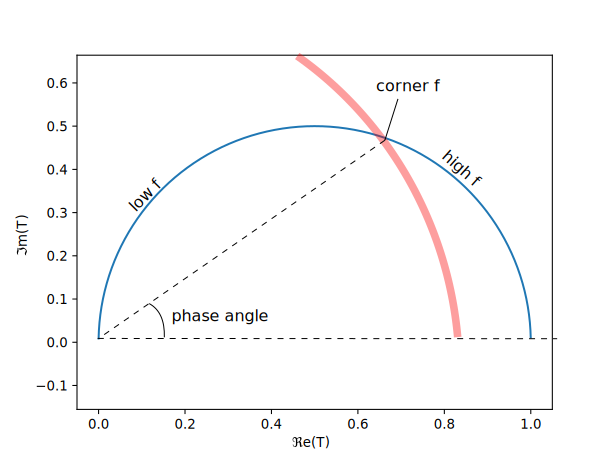
\includegraphics[width=\columnwidth]{images/nyquist_annotated}
  \caption{The thin solid line in the complex plane is the Nyquist
    plot. Each point on this line is the real and imaginary part of
    $\mathbf{T} = T(\cos(\phi)+ i \sin(\phi))$ at a particular
    frequency. The thick solid line represents the
    $\mbox{abs}(\mathbf{T})=1/\sqrt{2}$, so the intersection of the
    solid lines represents the corner frequency. The angle is the
    phase shift of the filter at this corner frequency.}
  \label{fig:nyquist}
\end{figure}

\section*{The Elvis II+ platform}
\begin{figure}
  \centering
  \includegraphics[width=\columnwidth]{images/elvisIIplus.jpg}
  \includegraphics[width=\columnwidth]{launcher.png}
  \caption{Top: photograph of the Elvis II+ board (top). Bottom: The
    graphical user interface or ``instrument launcher,'' containing
    such useful devices as the digital multimeter (DMM), an
    oscilloscope (Scope), a function generator (FGEN) and a Bode
    analyser (Bode).}
  \label{fig:elvisii}
\end{figure}
We will build circuits that act as a filter to an oscillatory input
signal on a platform from National Instruments called the ``Elvis
Board'' (see the top panel of Figure~\ref{fig:elvisii}). The breadboard of
the Elvis Board allows circuits to be tested without having to use
solder to connect components. Furthermore, the Elvis Board contains a
function generator to apply an oscillating voltage to put into your
circuit, and also a digital oscilloscope to interrogate the output of
the signal that runs through your circuit. A USB cable connects the
ELVIS II+ board to a PC with the appropriate software installed (the
GUI is shown in the bottom of Figure~\ref{fig:elvisii}), so you can
control the function generator, the oscilloscope settings, and display
the outputs.  To access these tools inside the Elvis board, ensure
that the USB plug is connected to a PC and the Elvis II+ is powered on
with the switch on the side of the device. The LED indicator for the
USB should display `READY'. You can now launch the GUI called `NI ELVISmx
Instrument Launcher'

In this experiment we will use the Elvis' built-in function generator
to drive a circuit built on the breadboard. The Bode plot analyzer
will be used to probe the voltage across the different components of
your circuit. The Elvis board has many options to build and test a
circuit. Here, we explain one way to set up your board. This requires
three connections to be made between the Elvis and the circuit board
under test:
\begin{itemize}
\item Activate the function generator by connecting two bare wires
  from pin 33 (FGEN on left hand plug board of ELVIS) and pin 49 (GND
  on left hand plug board of ELVIS) to the input of the circuit you
  wish to test using alligator clips.
\item Connect a BNC cable with alligator clips between oscilloscope
  channel 0 (top left hand side of the Elvis) and the input of the
  circuit you wish to test. The black lead goes to ground, and the lead with the
  other colour (blue, or red) is the positive.
\item Connect a BNC cable with alligator clips between
  oscilloscope channel 1 (top left hand side of the Elvis) and the
  output of the circuit you wish to test. The black lead goes to
  ground, the other colour is positive.
\item Launch the Bode function analyzer program from the GUI to
  measure Bode amplitude and phase plots over a frequency
  range defined in the GUI.
\end{itemize}

\noindent\textbf{Note:} Save
your data from the graphical user interface of the ELVIS board, under
the ``log'' button. You can then import your data into Python to
analyse and plot the results. Save these plots for your report. There
are many ways to import the data in python, but one of our favourites
is using the pandas package. All python packages you need are
installed on the lab computers, or you can use Google's COLAB to do
your computing in the Cloud.

\section*{Experiments}
In this lab, you will explore two types of passive filters: RC and LC
filters. The former contains a circuit made of resistors (R) and
capacitors (C), while the latter is a circuit with inductor(s) L and
capacitor(s) C. 

\subsubsection*{RC Filters}
The simplest of filters is one with a resistor $R$ and a capacitor $C$
in series (Figure~\ref{fig:filterAB}). Such a circuit acts as a
filter, because the impedance of a capacitor is frequency
dependent. Let us explore both experimentally and theoretically the
filtering capabilities of this simple circuits.

\begin{itemize}
\item build the circuit of Figure~\ref{fig:filterAB} with a resistor
  $R=10~k\Omega$ and a capacitor $C=22$~nF on your Elvis board.
\item Set the function generator on your Elvis board to sweep the
  input voltage from 100 Hz to 1MHz. 
\item Measure the ratio of the voltage across the resistor $R$ over
  the input voltage with the Bode Analyser on your Elvis Board. What
  is this ratio called?
\item Save your data and plot these in python as a phase and
  magnitude Bode plot.
\end{itemize}

In PHYS121 you learned that the impedance of the capacitor can be
written as $Z_c= 1/(j\omega C),$ where $j$ is the imaginary unit, and
$\omega = 2\pi f$ is the angular frequency.

\begin{enumerate}
\item Explain in your report why the voltage drop across the resistor
  in the circuit of Figure~\ref{fig:filterAB} is a fraction of the
  input voltage:
  $$\mathbf{V}_{out}(\omega)=
  \frac{R}{R+{\frac {1}{j\omega C}}}\mathbf{V}_{in}(\omega).$$
  % Apply Kirchhof's Law: the voltage drop over the two components
  % needs to add to the input voltage.
\end{enumerate}
\begin{figure}
  \centering
  \includegraphics[width=\columnwidth]{images/RCfilter}
  \caption{Circuit diagram of filters A and B. The input is $V_{in}$,
    and the outputs are $V_{out,A}$ for filter A, and $V_{out,B}$ for
    filter B.}
  \label{fig:filterAB}
\end{figure}

The transfer function of Filter A is then
\begin{equation}
  \mathbf{T}_A=\frac{\mathbf{V}_{out, A}}{\mathbf{V}_{in}}=
  \frac{R}{R+1/(\mathrm{j}\omega C)}=\frac{1}{1-\mathrm{j}\omega_0/\omega},
\end{equation}
where
\begin{equation}
  \omega_0=\frac{1}{RC}.
\end{equation}
\begin{enumerate}
\item Based on what you read so far in this hand-out, show that
  $\omega_0 = 1/RC$ is the cutoff, or corner, angular
  frequency. % if $\omega = \omega_0$, then $T_A = 1/\sqrt{2}$.
  
\item What is $\omega_0$ for Filter~A?
  
\item Use Python to plot a theoretical Bode amplitude plot (in
  dB) and Bode phase plot (in degrees) on the same figure, using a
  frequency range of 100Hz-1MHz.
  
\item On a separate figure, use Python to
  construct a theoretical Nyquist plot from your data.
  
\item Explain why the output voltage measured
  across the resistor is almost zero for very low
  frequencies. %impedance of capacitor dominates. Oral exam question:
  % what happens when you have a very large value of $R$?
\item What sort of output waveform ($\mathbf{V}_{out}$) would you
  expect to see on an oscilloscope from this filter when using a 1kHz
  square wave as your input waveform
  ($\mathbf{V}_{in}$)? % The flat parts of the square wave are DC-like
  % and filtered to zero. Only the sharp changes
  % contain high f and remain, leaving a saw-tooth
  % pattern.
\end{enumerate}

Filter A, as shown in Figure~\ref{fig:filterAB}, is a simple high-pass
phase-advance filter, commonly used for inter-stage coupling where DC
isolation is required.  High pass filters are characterised by their
ability to allow high frequencies to pass through the filter while
suppressing low frequencies.

We can also consider the voltage measured over the capacitor in the
same circuit as the output ($\mathbf{V}_{out, B}$ in
Figure~\ref{fig:filterAB}).  This output is
\begin{equation}
  \mathbf{V}_{out, B}(\omega)={\frac {\frac {1}{j\omega C}}{R+{\frac {1}{j\omega C}}}}\mathbf{V}_{in}(\omega)={\frac {1}{1+RCj\omega}}\mathbf{V}_{in}(\omega) =
  {\frac {1}{1+j\omega/\omega_0}}\mathbf{V}_{in}(\omega)
\end{equation}
and the transfer function for Filter B is then
\begin{equation}
  \mathbf{T}_B =
  \frac{\mathbf{V}_{out, B}}{\mathbf{V}_{in}}=
  \frac{1}{1+\mathrm{j}\omega/\omega_0}.
\end{equation}
\begin{enumerate}
\item Make Bode plots of the theoretical and experimental transfer
  function $\mathbf{T}_B$.
\end{enumerate}

Because the circuit used for Filters A and B is the same, the output for
Filter B can also be derived from the output of Filter A:
\begin{equation}
  \mathbf{V}_{in}(f)=\mathbf{V}_C(f)+\mathbf{V}_R(f)
\end{equation}
Therefore,
\begin{equation}
  \mathbf{T}_B(f) =\frac{\mathbf{V}_C(f)}{\mathbf{V}_{in}(f)}
  =\frac{\mathbf{V}_{in}(f)-\mathbf{V}_R(f)}{\mathbf{V}_{in}(f)}
  =1-\frac{\mathbf{V}_R(f)}{\mathbf{V}_{in}(f)}
  =1-\mathbf{T}_A(f).
\end{equation}

\begin{enumerate}
\item Construct Bode amplitude and phase plots with Filters A and B in
  each panel.
\item As the voltage transfer function $\mathbf{T}_B$ can be derived
  from the voltage transfer function for Filter A, construct a Nyquist
  plot by by adding $-\mathbf{T}_A$ to $\mathbf{1}$ vectorially. This
  vector addition is equivalent to addition of complex numbers.
\item Discuss how the Bode and Nyquist plots inform us about the relations
  between these two filters.
\end{enumerate}
Based on your measurements and theoretical calculations, Filter B in
the circuit in Figure~\ref{fig:filterAB} is a simple low-pass
phase-delay filter used to remove unwanted high-frequency signals.

\section{LC filters}
We now saw that RC filters act as high- or low-pass filters. If we
replace the resistor $R$ with a inductor $L$, we have an LC circuit.
We will see that LC filters are able to act as an electrical
resonator. These resonant properties can be used to select certain
frequencies out of a range of frequencies, making them useful for
applications such as tuning radio transmitters and receivers.

{\bf HERE?} Theoretical LC filters are unachievable in the real world,
as the capacitor and inductor combination will always possess some
resistance, and the output signal will be damped even at resonance.

{\bf HERE?} The \textbf{Q factor} (or quality factor) is a measure of the
``sharpness'' of the resonance. Conversely, it determines how damped
an oscillator is. The definition of $Q$ is the full width at half of
the maximum value. See experiment 263 and its handout for more
details. The $Q$ of an LC filter is not infinite due to the internal
resistance of the inductor and capacitor combination. EQUATION HERE. A
circuit having a low Q factor (Q$<1/2$) is said to be overdamped, and
will not oscillate. A circuit with a high Q factor (Q$>1/2$) is said
to be underdamped and will oscillate with a decay of the amplitude of
the signal. When Q$=1/2$ the circuit is said to be critically damped.

\subsection{Filter C}
\begin{figure}
  \centering
  \includegraphics[width=0.7\textwidth]{images/filterC.png}
  \caption{Circuit diagram for filter C (left) and experimental setup
    (right).}
  \label{fig:lc1}
\end{figure}
The circuit shown in Fig. \ref{fig:lc1} shows a real LC circuit, with
the resistance $R_p$ representing the resistance from the inductor and
capacitor in parallel. The voltage transfer function for this circuit
is given by:
\begin{equation}
  \mathbf{T}_C=\frac{\mathbf{V}_{out}}{\mathbf{V}_{in}}=\frac{R_2}{R_2+z_p},
\end{equation}
where the impedance of the parallel components is 
\begin{equation}
  z_p\equiv \frac{1}{1/Z_R+1/Z_C+1/Z_L}=\frac{R_p}{1+\mathrm{j}R_p\left(\omega C - \frac{1}{\omega L}\right)}.
\end{equation}
It is clear that $|\mathbf{T}_C|$ is a minimum when $|z_p|$ is a
maximum. This will occur at the resonant
frequency, %where $\omega=\omega_0=1/\sqrt{LC}$, i.e.\ at the frequency
$\omega_0=1/\sqrt{LC}$.

We can define $Q_p$ as the Q factor of the parallel inductor-capacitor
combination, which gives a measure of how damped the system is. $Q_p$
is given by
\begin{equation}
Q_p=\frac{R_p}{\omega_0 L}=\omega_0 R_p C.
\end{equation}

The Q factor of filter C (different from $Q_p$) can then be defined as
\begin{equation}
  Q_C=Q_p\sqrt{1-2|\mathbf{T}_{Cmin}|^2},
\end{equation}
where $|\mathbf{T}_{Cmin}|$ is the minimum value of $|\mathbf{T}_C|$.

\begin{enumerate}
\item[(6)] The resistance $R_p$ of filter C (see Fig. \ref{fig:lc1})
  is the parallel loss resistance of the inductor (the capacitor has
  negligible loss resistance).  Set $R_2$ to have a value of
  $300\Omega$ and use the Elvis to obtain a Bode plot for the filter.
  
\item[(7)] Determine the frequencies $f_{min}$ and $f_{max}$
  corresponding to the greatest positive and negative phase shifts
  between the input and output signals. %approx 2.6kHz and 42kHz
  
\item[(8)] Use this plot to find the value of $R_p$, and hence
  determine $Q_p$. Find the value of $Q_C$, and interpret it in
  relation to the damping of the circuit.

\item[(9)] Using your knowledge of the resistances in this circuit,
  obtain a theoretical Bode plot for this filter with Python. Confirm
  that it agrees with what you have found experimentally.

\item[(10)] Create a Nyquist plot containing both theoretical and
  experimental data, and see whether the two agree.
\end{enumerate}

\subsection{Filter D}
\begin{figure}[ht]
  \centering
  \includegraphics[width=0.8\textwidth]{images/filterD.png}
  \caption{Circuit diagram for filter D (left) and experimental setup (right).}
  \label{fig:lc2}
\end{figure}
In the circuit of Filter D (see Fig. \ref{fig:lc2}), $R_s$ represents
the power loss resistance of the inductor-capacitor series
combination. The voltage transfer function of Filter D is given by:
\begin{equation}
  \mathbf{T}_D=\frac{\mathbf{V}_{out}}{\mathbf{V}_{in}}=\frac{R_1}{R_1+z_s},
  \label{eq:D1}
\end{equation}
where
\begin{equation}
  z_s=R_s\left[1+\mathrm{j}\left(\frac{\omega L}{R_s}-\frac{1}{\omega R_s C}\right)\right].
  \label{eq:D2}
\end{equation}
From equation \ref{eq:D1}, we can see that $\mathbf{T}_D$ is a maximum
when $z_s$ is a minimum, and equation \ref{eq:D2} shows us that this
occurs at the resonant frequency, when $\omega=\omega_0
=1/\sqrt{LC}$. If we define $Q_s$ to be the quality factor of the
series inductor-capacitor combination, then by definition
\begin{equation}
  Q_s =\frac{\omega_0 L}{R_s}=\frac{1}{\omega_0 R_s C}.
\end{equation}
The Q factor of filter D is given by:
\begin{equation}
  Q_D=\frac{\omega_0 L}{R_1 + R_s}=\frac{1}{\omega_0(R_1+R_s)C}=Q_s\frac{R_s}{R_1}|\mathbf{T}_{Dmax}|.
\end{equation}

\begin{enumerate}
\item[(11)] Use the Elvis to obtain an experimental Bode plot for the
  circuit shown in Fig. \ref{fig:lc2}.

\item[(12)] Find $R_s$ and hence determine the value of $Q_s$. Find
  the value of $Q_D$ and interpret this in relation to how damped the
  circuit is.

\item[(13)] Use Python to construct a theoretical Bode plot and a
  Nyquist plot for this circuit, using your experimental values for
  the circuit components. Check whether these agree with the
  experimental plots.

\end{enumerate}


S. Ruddell, S. Murdoch February 2013

S. Coen 2021

K. van Wijk, 2022
\end{document}


